\section{Experiments}
\label{sec:experiments}

We organize our empirical study around three questions: where AHE sits on the map of existing approaches to harness design, whether what it produces is portable beyond its optimization target, and what inside the loop drives the gain.

\begin{tcolorbox}[
    colback=blue!3,
    colframe=blue!40,
    arc=2pt,
    boxrule=0.5pt,
    left=6pt, right=6pt, top=4pt, bottom=4pt,
    title={\textbf{Research Questions}},
    fonttitle=\bfseries,
    coltitle=black,
    colbacktitle=blue!10
  ]
  \begin{enumerate}
    \setlength{\leftmargini}{1.5em}
    \setlength{\itemsep}{2pt}
    \setlength{\parsep}{0pt}
      \item \textbf{RQ1} (\S\ref{sec:experiments:main})\textbf{: Why agentic harness engineering, rather than human-engineered harnesses or other automated methods?}
      \item \textbf{RQ2} (\S\ref{sec:experiments:transfer})\textbf{: Does agentic harness engineering overfit to its optimization target?}
      \item \textbf{RQ3} (\S\ref{sec:experiments:mechanism})\textbf{: What inside AHE drives its gains, and how reliable is the loop's self-attribution?}
  \end{enumerate}
\end{tcolorbox}

\subsection{Setup}
\label{sec:experiments:setup}

\paragraph{Evaluation.}
\label{sec:experiments:metrics}
We drive evolution on the full 89 tasks of Terminal-Bench 2~\citep{merrillTerminalBenchBenchmarkingAgents2026a}, split as 4 easy, 55 medium, and 30 hard, with per-task timeout extended to 1 hour. For cross-benchmark transfer we evaluate the AHE harness on SWE-bench-verified~\citep{jimenezSWEbenchCanLanguage2023}, 500 tasks across seven repositories. 
We report two metrics per configuration: \textit{pass@1}, the mean binary success rate over $k$ rollouts per task; and \textit{tokens/trial}, the mean per-trial total of prompt plus completion tokens across all LLM calls, in thousands. Infrastructure-aborted or timed-out trials count as failures under pass@1 (matching the official terminal-bench leaderboard) and are excluded from token means to avoid truncated figures. Runtime infrastructure (framework, dispatcher, sandbox, tracer, and concurrency) is detailed in Appendix~\ref{app:setup}.

\paragraph{Models.}
For both the evolution loop and the main experiment of \S\ref{sec:experiments:main}, all three role agents (the Code Agent, the Agent Debugger, and the Evolve Agent) share one base model, GPT-5.4~\citep{openaiIntroducingGPT542026} at the high reasoning setting. 
% Fixing the model across roles isolates the effect of harness edits from confounds introduced by a different analyzer or editor. 
For cross-model transfer (\S\ref{sec:experiments:transfer}), we re-evaluate the Code Agent on five alternate bases: GPT-5.4~\citep{openaiIntroducingGPT542026} at medium and xhigh reasoning, qwen-3.6-plus~\citep{teamQwen36PlusRealWorld2026,yangQwen3TechnicalReport2025a}, gemini-3.1-flash-lite-preview~\citep{googleGemini31FlashLiteModelCard2026}, and deepseek-v4-flash~\citep{DeepSeek_V4pdfDeepseekaiDeepSeekV4Pro2026}.

\subsection{RQ1: Main Results}
\label{sec:experiments:main}

% \input{figures/evolution-curve}

% \begin{table}[htbp]
%     \centering
%     \footnotesize
%     \setlength{\tabcolsep}{6pt}
%     \renewcommand{\arraystretch}{1.05}
%     \caption{Pass@1 on Terminal-Bench 2 across 89 tasks, by official difficulty. \textbf{NexAU\textsubscript{0}} is the shared seed; ACE, TF-GRPO, and \textbf{AHE} are three self-evolution loops layered on top of it. Bold marks the best per column; ties are all bold.}
%     \label{tab:main-results}
%     \begin{tabular}{lcccc}
%         \toprule
%         Method & All & Easy & Med. & Hard \\
%                & {\scriptsize 89} & {\scriptsize 4} & {\scriptsize 55} & {\scriptsize 30} \\
%         \midrule
%         \rowcolor{gray!20} \multicolumn{5}{l}{\textit{Human-designed harness}} \\
%         opencode               & 47.2\% & 75.0\% & 52.7\% & 33.3\% \\
%         terminus-2             & 62.9\% & 75.0\% & 74.5\% & 40.0\% \\
%         Codex                  & 71.9\% & 75.0\% & 80.0\% & \textbf{56.7\%} \\
%         \addlinespace
%         \rowcolor{gray!20} \multicolumn{5}{l}{\textit{Self-evolved from NexAU\textsubscript{0}}} \\
%         NexAU\textsubscript{0} & 69.7\% & 87.5\% & 78.2\% & 51.7\% \\
%         ACE                    & 68.9\% & 91.7\% & 78.2\% & 48.9\% \\
%         TF-GRPO                & 72.3\% & \textbf{100.0\%} & 79.4\% & 55.6\% \\
%         \textbf{AHE}           & \textbf{77.0\%} & \textbf{100.0\%} & \textbf{88.2\%} & 53.3\% \\
%         \bottomrule
%     \end{tabular}
% \end{table}
\setlength{\intextsep}{2pt}
\setlength{\columnsep}{8pt}
\begin{wraptable}{r}{0.5\linewidth}
    \centering
    \footnotesize
    \setlength{\tabcolsep}{4pt}
    \renewcommand{\arraystretch}{1.0}
    \setlength{\abovecaptionskip}{2pt}
    \setlength{\belowcaptionskip}{2pt}
    \caption{Pass@1 on Terminal-Bench 2 across 89 tasks, by official difficulty. NexAU\textsubscript{0} is the shared seed; ACE, Training-Free GRPO, and \textbf{AHE} are three self-evolution loops layered on top of it. Bold marks the best per column; ties are all bold.}
    \label{tab:main-results}
    \begin{tabular}{lcccc}
        \toprule
        Method & All & Easy & Med. & Hard \\
               & {\scriptsize 89} & {\scriptsize 4} & {\scriptsize 55} & {\scriptsize 30} \\
        \midrule
        \rowcolor{gray!20} \multicolumn{5}{l}{\textbf{Human-designed harness}} \\
        OpenCode               & 47.2\% & 75.0\% & 52.7\% & 33.3\% \\
        Terminus-2             & 62.9\% & 75.0\% & 74.5\% & 40.0\% \\
        Codex              & 71.9\% & 75.0\% & 80.0\% & \textbf{56.7\%} \\
        \addlinespace
        \rowcolor{gray!20} \multicolumn{5}{l}{\textbf{Self-evolved from NexAU\textsubscript{0}}} \\
        NexAU\textsubscript{0} & 69.7\% & 87.5\% & 78.2\% & 51.7\% \\
        ACE                    & 68.9\% & 91.7\% & 78.2\% & 48.9\% \\
        TF-GRPO                & 72.3\% & \textbf{100.0\%} & 79.4\% & 55.6\% \\
        \textbf{AHE}           & \textbf{77.0\%} & \textbf{100.0\%} & \textbf{88.2\%} & 53.3\% \\
        \bottomrule
    \end{tabular}
\end{wraptable}

We run a single AHE campaign of ten iterations from the bash-only \textbf{NexAU\textsubscript{0}} seed (\S\ref{sec:method:harness}) on Terminal-Bench 2, finishing in roughly 32 hours; the best resulting configuration is reported as \textbf{AHE}. The two self-evolve baselines ACE~\citep{zhangAgenticContextEngineering2025a} and Training-Free GRPO (TF-GRPO)~\citep{caiTrainingFreeGroupRelative2025} start from the same NexAU\textsubscript{0} seed.

\paragraph{AHE outperforms both human-designed and self-evolve baselines.}
AHE outperforms every baseline on our panel: three human-designed harnesses, OpenCode~\citep{anomalyOpencodeOpenSource2025}, Terminus-2~\citep{harborTerminus22026}, and Codex~\citep{openaiCodexCLI2025}, and the two self-evolve baselines.
Figure~\ref{fig:training_curve} shows the gain accumulates across iterations, with continued evolution pushing pass@1 further above the NexAU\textsubscript{0} seed.
By difficulty, the only exception is the Hard tier, where AHE marginally trails Codex. We trace this gap to interference between AHE's components on long-horizon tasks rather than to a missing capability: swapping AHE's long-term memory alone into the NexAU\textsubscript{0} seed, without the other AHE components, already surpasses Codex on Hard (\S\ref{sec:experiments:rq3a}).

\paragraph{Prompt-only self-evolution misses the components that carry AHE's gain.}
The gaps to ACE and TF-GRPO trace to a layer mismatch. ACE distills natural-language playbooks the agent reads in-context, and TF-GRPO is a trajectory-feedback variant of GRPO that reinforces successful tool sequences; neither method opens the surrounding scaffolding to edits.
AHE instead jointly evolves system prompt, tools, middleware, and long-term memory, and \S\ref{sec:experiments:rq3a} shows the gain concentrates in the latter three components, exactly the layers ACE and TF-GRPO leave untouched.

\subsection{RQ2: Transfer to Unseen Tasks and Base Models}
\label{sec:experiments:transfer}

AHE's harness is evolved on Terminal-Bench 2 with GPT-5.4 high. We probe whether it encodes general coding-agent experience or overfits to that target by transferring the evolved harness unchanged, without further evolution, to two off-target settings: a different task surface (SWE-bench-verified) and three alternate base models.

\begin{table}[t]
    \centering
    \small
    \setlength{\tabcolsep}{5pt}
    \renewcommand{\arraystretch}{1.05}
    \caption{Cross-benchmark transfer on SWE-bench-verified. ACE, Training-Free GRPO (TF-GRPO), and \textbf{AHE} share the \textbf{NexAU\textsubscript{0}} seed and differ only in their self-evolution loop; all four columns run on GPT-5.4. AHE and the two self-evolve baselines are evolved on Terminal-Bench 2 and evaluated without in-domain re-evolution. Per-column bold marks the best; ties are all bold.}
    \label{tab:swe-verified-analysis}
    \begin{tabular}{lc @{\hspace{10pt}} cccc @{\hspace{10pt}} cccc}
        \toprule
         &  & \multicolumn{4}{c}{Success rate $\uparrow$} & \multicolumn{4}{c}{Tokens k $\downarrow$} \\
        \cmidrule(lr){3-6} \cmidrule(lr){7-10}
        Repo & $N$
        & ACE & TF-GRPO & NexAU\textsubscript{0} & \textbf{AHE}
        & ACE & TF-GRPO & NexAU\textsubscript{0} & \textbf{AHE} \\
        \midrule
        All            & 500 & 74.6\% & 74.2\% & 75.2\% & \textbf{75.6\%} & 679 & 582 & 526 & \textbf{461} \\
        \midrule
        django         & 231 & 79.2\% & 78.8\% & 79.2\% & \textbf{81.0\%} & 707 & 583 & 527 & \textbf{484} \\
        sympy          &  75 & 69.3\% & 68.0\% & \textbf{70.7\%} & \textbf{70.7\%} & 602 & 572 & 494 & \textbf{479} \\
        sphinx-doc     &  44 & 61.4\% & 65.9\% & 68.2\% & \textbf{70.5\%} & 990 & 848 & 731 & \textbf{656} \\
        matplotlib     &  34 & 70.6\% & 70.6\% & \textbf{73.5\%} & \textbf{73.5\%} & 622 & 530 & 486 & \textbf{391} \\
        scikit-learn   &  32 & \textbf{93.8\%} & \textbf{93.8\%} & \textbf{93.8\%} & 87.5\% & 451 & 378 & 307 & \textbf{257} \\
        pydata         &  22 & \textbf{77.3\%} & \textbf{77.3\%} & \textbf{77.3\%} & 72.7\% & 563 & 516 & 386 & \textbf{338} \\
        astropy        &  22 & \textbf{59.1\%} & \textbf{59.1\%} & 54.5\% & 50.0\% & 546 & 470 & 667 & \textbf{277} \\
        \bottomrule
    \end{tabular}
\end{table}


\paragraph{Cross-benchmark transfer.}
We evaluate the AHE harness on SWE-bench-verified against the seed and the two self-evolve baselines (NexAU\textsubscript{0}, ACE, TF-GRPO) under identical infrastructure (Table~\ref{tab:swe-verified-analysis}).

ACE and TF-GRPO both regress below the NexAU\textsubscript{0} seed in aggregate success while spending $11\%$ to $29\%$ more tokens than the seed: the playbook ACE injects and the trajectory distribution TF-GRPO reinforces were distilled on Terminal-Bench 2 traces and ride the prompt at every model call, so on a different task surface that text adds cost without reshaping the underlying policy.

AHE instead achieves the highest aggregate, with the seed-relative gain concentrating on django and sphinx-doc, the two largest and most token-expensive repositories whose multi-step edit-and-verify loop matches the structure AHE's tools, middleware, and long-term memory compress on Terminal-Bench 2.
Marginal regressions appear only on the three smallest repositories, consistent with pass@1 variance on small repos exceeding the per-repo gain.
AHE also cuts aggregate tokens by $32\%$ against ACE, $21\%$ against TF-GRPO, and $12\%$ against the seed: encoding behavior in tools, middleware, and memory avoids the per-call re-derivation cost prompt-only baselines incur.

\begin{figure}[t]
    \centering
    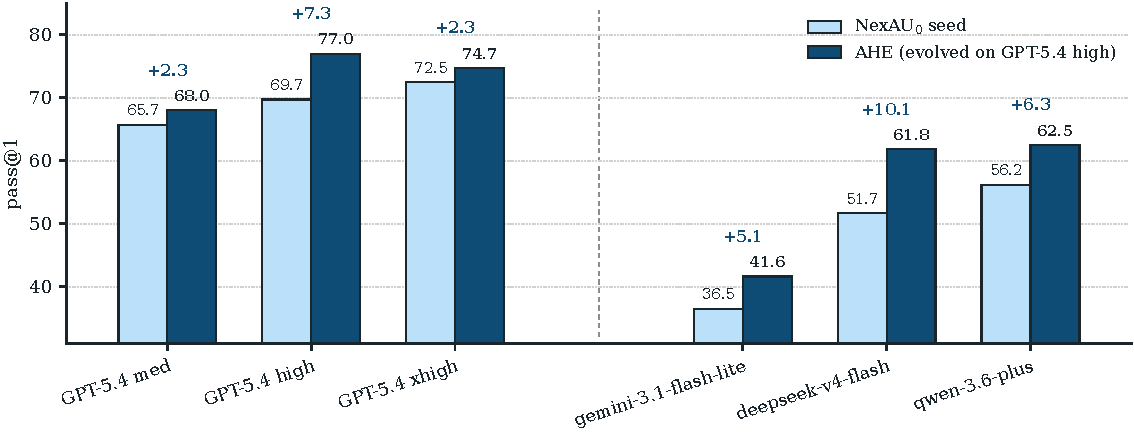
\includegraphics[width=0.9\linewidth]{figures/transfer_model.pdf}
    \caption{Cross-model transfer on Terminal-Bench 2, 89 tasks. The AHE workspace evolved on GPT-5.4 high is re-evaluated on each base without further evolution, paired against the NexAU\textsubscript{0} seed on the same base. All bases gain over the seed, with cross-family bases gaining more than within-family ones.}
    \label{fig:transfer-model}
\end{figure}


\paragraph{Cross-model transfer.}
We re-evaluate both the NexAU\textsubscript{0} seed and AHE on the five alternate bases listed in \S\ref{sec:experiments:setup}. Figure~\ref{fig:transfer-model} reports five positive pass@1 gains from $+2.3$ to $+10.1$\,pp.

Cross-family gains dominate within-family ones: deepseek-v4-flash moves $+10.1$\,pp from $51.7\%$ to $61.8\%$, qwen-3.6-plus $+6.3$\,pp from $56.2\%$ to $62.5\%$, and gemini-3.1-flash-lite-preview $+5.1$\,pp from $36.5\%$ to $41.6\%$, all above the $+2.3$\,pp on GPT-5.4 medium and xhigh. We read this as bases further from saturation leaning more on the coordination patterns AHE has fixed inside tools, middleware, and long-term memory, while a stronger base re-derives the same coordination from its prompt at low marginal cost.

Within one family the profile is non-monotone: $+2.3$\,pp on medium, $+7.3$\,pp on high from \S\ref{sec:experiments:main}, and $+2.3$\,pp on xhigh. AHE's step budget and per-task timeout were fitted to GPT-5.4 high during evolution; medium has more time-per-step slack but loses a reasoning tier of raw capability, while xhigh pushes more trials past the per-task timeout, which our pass@1 convention (\S\ref{sec:experiments:metrics}) counts as failures. Either direction discounts the gain.

The headline finding is that all five gains land positive: the AHE workspace is not specific to one provider's idioms or one reasoning depth. Their magnitude tracks the evolution operating point rather than raw base capability, so we treat the timeout-budget coupling as a generalization hazard discussed in our \nameref{sec:limitations} section.

\subsection{RQ3: Analysis}
\label{sec:experiments:mechanism}

We analyze the loop along two architectural choices that \S\ref{sec:method} places weight on: decomposed components (\S\ref{sec:experiments:rq3a}) and self-declared attribution (\S\ref{sec:experiments:rq3b}).


\subsubsection{RQ3a: where value accumulates across components}
\label{sec:experiments:rq3a}


Table~\ref{tab:ablations} decomposes the AHE gain at the component level by isolating one of the four evolved layers, long-term memory, tools, middleware, or system prompt, while holding the other three at their seed defaults. Three of the four single-component variants outperform the seed; the system-prompt swap is the only regression.

\begin{table}[htbp]
    \centering
    \small
     \vspace{\baselineskip}
    \caption{Component-level ablations on Terminal-Bench 2. Each ``+\,X only'' row swaps a single AHE component into the NexAU\textsubscript{0} seed; per-column best is bolded. Most single-component swaps already beat the seed, and the single-component gains overshoot full AHE's aggregate, indicating components interact non-additively rather than stacking cleanly.}
    \label{tab:ablations}
    \begin{tabular}{lcccc}
        \toprule
        Variant & All & Easy & Medium & Hard \\
                & {\scriptsize 89 tasks} & {\scriptsize 4 tasks} & {\scriptsize 55 tasks} & {\scriptsize 30 tasks} \\
        \midrule
        NexAU\textsubscript{0} & 69.7\% & 87.5\% & 78.2\% & 51.7\% \\
        \addlinespace
        + memory only         & 75.3\% & 50.0\% & 83.6\% & \textbf{63.3\%} \\
        + tool only           & 73.0\% & 75.0\% & 87.3\% & 46.7\% \\
        + middleware only     & 71.9\% & \textbf{100.0\%} & 81.8\% & 50.0\% \\
        + system\_prompt only & 67.4\% & 75.0\% & 78.2\% & 46.7\% \\
        \addlinespace
        \textbf{AHE} full     & \textbf{77.0\%} & \textbf{100.0\%} & \textbf{88.2\%} & 53.3\% \\
        \bottomrule
    \end{tabular}
\end{table}


\paragraph{Each component owns a different failure surface.}
Memory adds 12 boundary-case lessons (performance margin, queued-over-limit cancellation, evaluator-style closure, source-packaging layout); on Hard the lessons lift it above full AHE, while on Easy they reduce to superfluous re-verification.
Tools become a 1364-line shell that auto-surfaces contract hints from files near each command; on Medium it lands within $0.9$\,pp of full AHE, while on Hard a built-in publish guard closes the loop too early.
Middleware adds a finish-hook that forces one evaluator-isomorphic closure check; on Easy it clears every task, while on Hard it inflates turn count.
The system prompt encodes 79 lines of universal discipline whose executability depends on the other three; inserted alone it scores $-2.3$\,pp aggregate.

\paragraph{Components interact non-additively, capping the aggregate gain.}
The three positive single-component gains sum to $+11.1$\,pp against full AHE's $+7.3$\,pp, and on Hard the memory-only variant exceeds full AHE: memory, middleware, and the system prompt all push toward the same closure-style verification, so stacking them spends turns on redundant re-checks within the long-horizon budget.
Since the evolve agent optimises an aggregate dominated by 55 Medium tasks, it converges to a Medium-heavy trade-off that returns part of the Hard memory effect, and we leave interaction-aware evolution to future work.

\subsubsection{RQ3b: how reliably the loop's self-attribution tracks reality}
\label{sec:experiments:rq3b}

Each evolution round, our evolve model produces a change manifest naming which Terminal-Bench 2 tasks it expects to fix in the next round and which it flags at risk of regression. We compare the round-$N{-}1$ prediction against the round-$N$ ground truth, computing standard precision and recall over the 89 tasks separately for fixes and regressions.

\paragraph{Evidence-driven targeting.}
The fix panel of \Cref{fig:pred-aggregate} shows the evolve model's targeting is evidence-driven rather than guesswork. Cross-iteration fix-precision of \textbf{33.7\%} and fix-recall of \textbf{51.4\%} sit roughly 5x above the random-prediction baselines of 6.5\% and 10.6\%, so each harness edit lands on a real, agent-anticipated target rather than on an arbitrary subset of the panel.

\begin{figure}[t]
    \centering
    \begin{minipage}{0.4\linewidth}
        \centering
        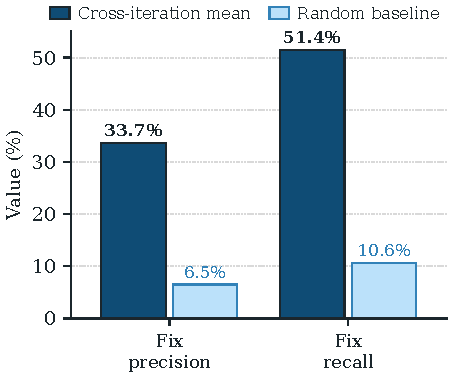
\includegraphics[width=\linewidth]{figures/summary_fix.pdf}
    \end{minipage}
    % \hfill
    \begin{minipage}{0.4\linewidth}
        \centering
        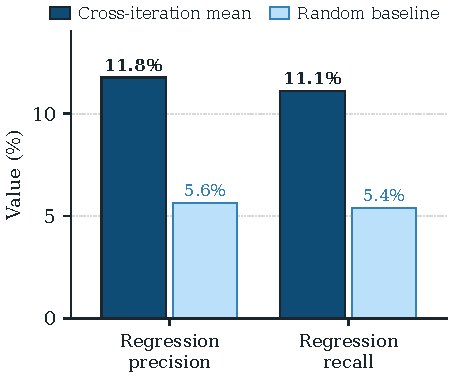
\includegraphics[width=\linewidth]{figures/summary_regression.pdf}
    \end{minipage}
    \caption{Cross-iteration mean precision and recall of the evolve model's self-predictions across 9 evaluation rounds of the GPT-5.4 AHE loop on Terminal-Bench 2, alongside the random-prediction baseline. Left: fix predictions. Right: regression predictions.}
    \label{fig:pred-aggregate}
\end{figure}

\paragraph{Regression blindness.}
The regression panel tells the opposite story: cross-iteration regression-precision of \textbf{11.8\%} and regression-recall of \textbf{11.1\%} sit only about 2x above their random baselines of 5.6\% and 5.4\%, so most upcoming regressions go unforeseen. The agent can justify why an edit should help, but it cannot reliably name the tasks the same edit is about to break, which is what produces the non-monotone steps in the evolution curve of \S\ref{sec:experiments:main}. Closing this gap is the clearest direction for future self-evolution loops. Appendix~\ref{sec:appendix:self-attribution} gives the per-round breakdown.
